\appendix

\section{ChronoInteract-82K Details}
\label{app:data_stats}

\paragraph{Construction pipeline.}
ChronoInteract-82K is built from public video-derived sources and benchmark materials.
We first filter videos for clear visual content and temporally locatable events, then extract chunk-level evidence and link facts that persist or change across chunks.
Given these aligned evidence chains, we use Qwen3.5-397B to generate candidate questions and reference answers from local facts and cross-chunk evidence.
Each candidate is assigned a query timestamp, an earliest answerable timestamp, and supporting evidence intervals, and is retained only after QA-quality and causal-consistency checks verify that the answer is supported by the causal context available at the answerable moment.

\paragraph{Statistics.}
Table~\ref{tab:data_stats} summarizes the current structured export.
It contains 4,812 streaming trajectories from 4,800 unique videos, with 82,335 finalized questions selected from 128,625 candidate task cards.
Each trajectory contains 17.1 questions on average.

\begin{table}[t]
  \centering
  \small
  \begin{tabular}{@{}lrrrr@{}}
    \hline
    Subset & Videos & Traj. & Questions & Q/T \\
    \hline
    SFT & 2,563 & 2,569 & 43,541 & 17.0 \\
    RL & 1,280 & 1,280 & 21,971 & 17.2 \\
    Val & 481 & 481 & 8,433 & 17.5 \\
    Test & 482 & 482 & 8,390 & 17.4 \\
    \hline
    \rowcolor{softblue}
    Total & 4,800 & 4,812 & 82,335 & 17.1 \\
    \hline
  \end{tabular}
  \caption{Statistics of the constructed streaming interaction data. Q/T denotes the average number of questions per trajectory.}
  \label{tab:data_stats}
\end{table}

\paragraph{Question distribution.}
Figure~\ref{fig:data_question_distribution} shows the distribution of constructed questions by streaming mode and task focus.
The inner ring groups examples into Real-Time, Backward Tracing, and Proactive interaction modes, while the outer ring shows the corresponding task focus under each mode.

\begin{figure}[t]
  \centering
  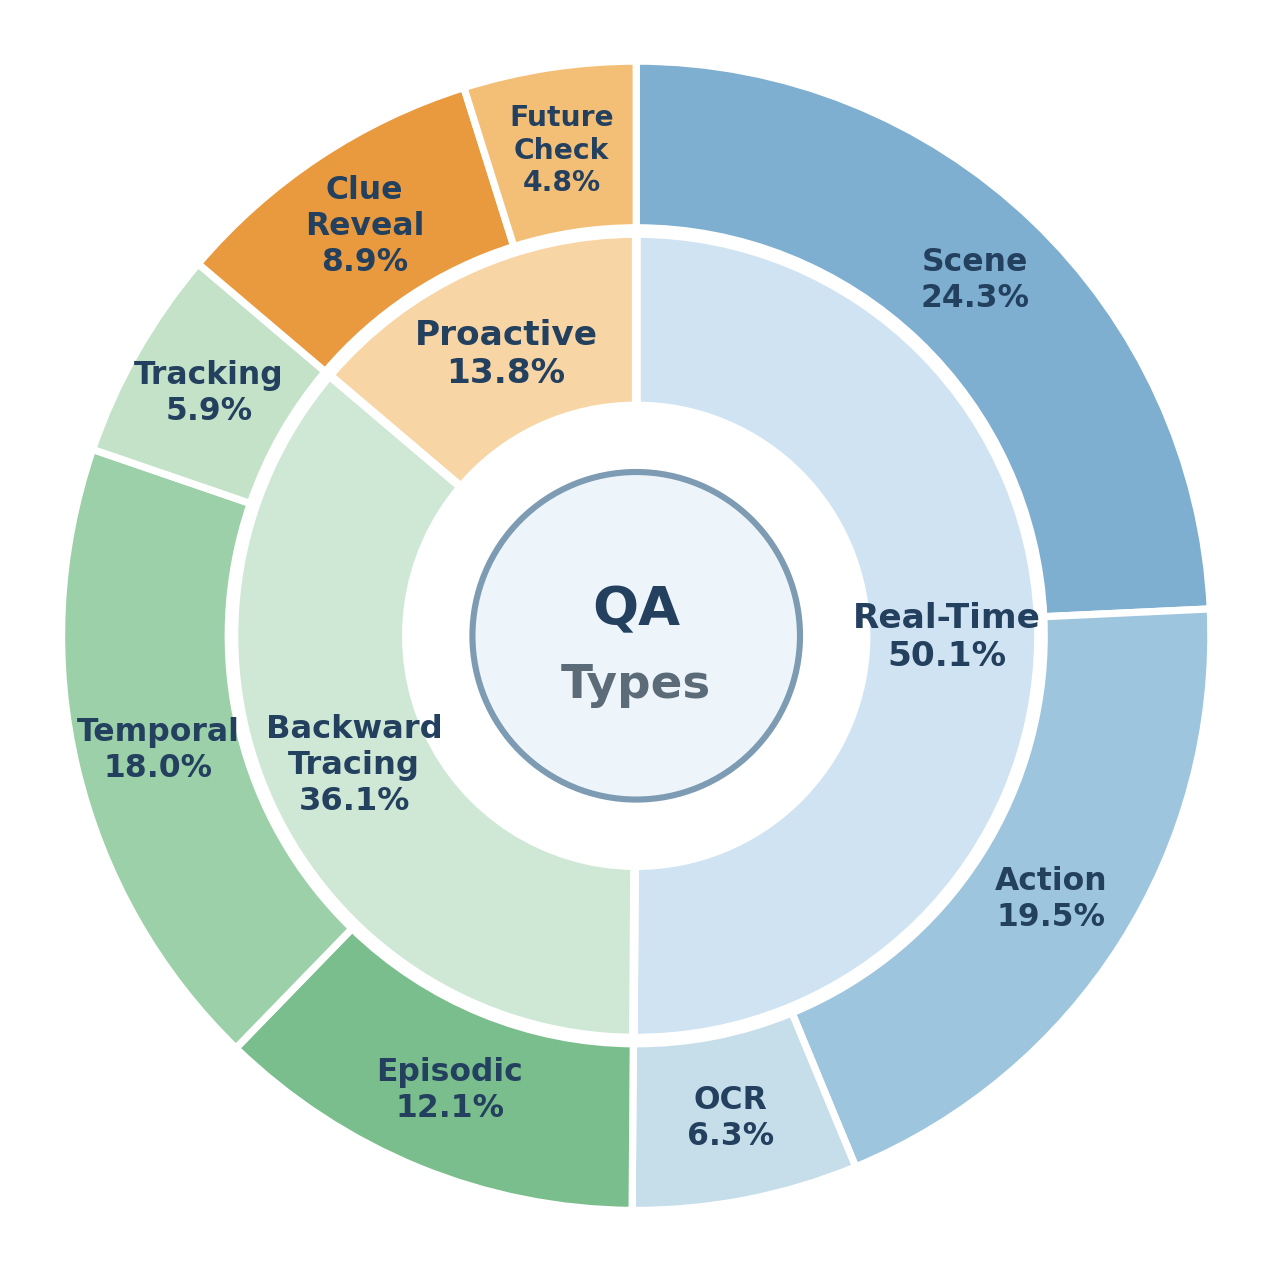
\includegraphics[width=0.92\columnwidth]{figures/figure_qa_distribution.png}
  \caption{Distribution of constructed questions by streaming mode and task focus.}
  \label{fig:data_question_distribution}
\end{figure}


\section{Streaming Protocol and Prompts}
\label{app:protocol_prompts}

\paragraph{Streaming protocol.}
WTI uses one message contract for data construction, SFT, RL rollout, and evaluation.
At each ordinary turn, the model receives the current timestamp \texttt{<t=N>}, the current 1-second video chunk, optional \texttt{<active\_query>} and \texttt{<response\_history>} blocks, and compact historical memory if available.
The current chunk is the only newly visible video evidence; earlier observations are represented by compact memory lines \texttt{<m t="start-end">summary</m>} or recovered through recall.
This contract keeps training and inference aligned with bounded KV-cache rollout: the model updates state online, makes one interaction decision per chunk, and never observes future frames.

\paragraph{Action and output grammar.}
The online action space contains three model-selected behaviors: stay silent, answer, or recall historical evidence; compact-memory updates are triggered by the system at memory-pressure boundaries.
For ordinary streaming turns, the assistant must begin with \texttt{<think>...</think>} and end with exactly one terminal action: \texttt{</Silence>} if no query should be answered, \texttt{</Response>} followed by an answer if the active query is answerable, or a Qwen-style tool call to \texttt{recall}.
Recall arguments are absolute source-video seconds, \texttt{start\_time} and \texttt{end\_time}, and the interval must be earlier than the current chunk.
The parser marks malformed outputs, multiple terminal actions, unsupported tool names, and future-looking recall ranges as action errors.

\paragraph{Prompt templates.}
Figure~\ref{fig:streaming_prompt_templates} shows the compact prompt templates used by the streaming agent.
The first prompt describes the causal streaming state and the allowed actions.
The second prompt is used only at memory-pressure boundaries; it asks the model to rewrite accumulated state into time-indexed memory lines without answering user questions or calling tools.

\begin{figure*}[t]
\centering
  \begin{minipage}[t]{0.48\textwidth}
  \begin{tcolorbox}[
    title=\textbf{System Prompt for WTI Streaming Actions},
    colback=gray!5,
    colframe=gray!60!black,
    boxrule=0.6pt,
    fonttitle=\bfseries,
    left=0.55em, right=0.55em, top=0.55em, bottom=0.55em,
    width=\linewidth
  ]
  \tiny
  \noindent\textbf{Role.}
  You are a streaming video reasoning assistant.
  The video arrives chunk by chunk; never use future frames.

  \medskip
  \noindent\textbf{Input State.}
  Each turn may contain the current timestamp, current frames, an active query, response history, compact memory, and recalled evidence.
  The current chunk is the only new visual input.

  \medskip
  \noindent\textbf{Available Actions.}
  \begin{enumerate}[leftmargin=*, noitemsep, topsep=2pt]
    \item \textbf{Silence}: use when no answer is ready or a query waits for future evidence.
    \item \textbf{Response}: use when the observed causal context is sufficient.
    \item \textbf{Recall}: use when a query needs older visual evidence outside the active window.
  \end{enumerate}

  \medskip
  \noindent\textbf{Recall Rule.}
  Use recall only for observed historical intervals.
  Arguments are absolute source-video seconds, \texttt{start\_time} and \texttt{end\_time}.
  Do not recall future ranges, duplicate prior recalls, or retrieve evidence already visible in current frames or memory.

  \medskip
  \noindent\textbf{Output Constraint.}
  Each turn must contain one \texttt{<think>} block and exactly one terminal action.
  For future-dependent questions, stay silent until the needed visual trigger is observed.
  \end{tcolorbox}
  \end{minipage}
  \hfill
  \begin{minipage}[t]{0.48\textwidth}
  \begin{tcolorbox}[
    title=\textbf{System Prompt for Compact-Memory Updates},
    colback=gray!5,
    colframe=gray!60!black,
    boxrule=0.6pt,
    fonttitle=\bfseries,
    left=0.55em, right=0.55em, top=0.55em, bottom=0.55em,
    width=\linewidth
  ]
  \tiny
  \noindent\textbf{Role.}
  You are updating compact video memory for a streaming video assistant.
  The input contains old memory, new captions, and the covered latest time span.
  Preserve useful old information and add observations that may support later questions.

  \medskip
  \noindent\textbf{Memory Rules.}
  \begin{enumerate}[leftmargin=*, noitemsep, topsep=2pt]
    \item Output only \texttt{<m t="start-end">summary</m>} memory lines.
    \item Use honest source-video time ranges; do not invent events outside the input.
    \item Merge adjacent complete units when possible, but do not repartition old ranges only for formatting.
    \item Preserve objects, people, actions, OCR, state changes, counts, and temporal order.
  \end{enumerate}

  \medskip
  \noindent\textbf{Forbidden Output.}
  Do not output JSON, Markdown, analysis, answers, tool calls, or \texttt{<think>} blocks.
  Return compact memory lines only.
  \end{tcolorbox}
  \end{minipage}
  \caption{Compact prompt templates used by WTI. Left: ordinary streaming action turns. Right: compact-memory update turns.}
  \label{fig:streaming_prompt_templates}
\end{figure*}

\section{Training, Rewards, and Implementation Details}
\label{app:implementation}

\paragraph{Training setting.}
WTI is trained with masked SFT followed by Stream-GDPO in the same chunk-level streaming environment used for evaluation.
The SFT stage initializes the action protocol, response timing, recall syntax, and compact-memory behavior from teacher trajectories.
The vision encoder is frozen, while the language model and multimodal projector are updated.
Supervision is applied only to assistant-generated tokens; stream inputs, user queries, environment observations, and recalled chunks are treated as context.

\paragraph{Stream-GDPO rollout.}
Stream-GDPO starts from the SFT checkpoint and rolls out one video stream with one or more timed questions.
The controller supplies the current chunk, active-query state, recall results, and compact-memory boundaries, while each model output updates the stream state before the next chunk.
The policy is optimized on assistant action turns with group-normalized trajectory advantages, so answer correctness, recall quality, and memory maintenance are credited within the same online trajectory.
This setup avoids a train-test mismatch between offline full-video supervision and bounded-context streaming inference.

\paragraph{Reward and rollout implementation.}
Question-level rewards cover answer outcome, format validity, response timing, and recall use.
Recall rewards favor historical intervals that overlap the supporting evidence and penalize future-looking or unnecessary recall.
The compact-memory reward is computed at the rollout level because a memory update is useful only if it preserves evidence for later turns.
Together, the reward terms train the model to answer from current evidence when possible, recall past evidence when needed, and keep enough time-indexed state for future questions.

\paragraph{Hyperparameters and compute.}
WTI is initialized from Qwen3-VL-8B-Instruct.
The stream is rendered as 1-second chunks at 2 FPS, and the active visual window contains 8 chunks, or 16 frames.
Recall returns up to 4 uniformly sampled chunks from the requested historical interval.
For masked SFT, we train chunk-level trajectories with learning rate \(1\times10^{-5}\).
For Stream-GDPO, we use veRL with prompt batch size 64 and sample 4 rollouts per prompt.
The actor learning rate is \(1\times10^{-5}\), asymmetric clipping uses \(\epsilon_{\mathrm{low}}=0.2\) and \(\epsilon_{\mathrm{high}}=0.28\), and the action-branch loss weight is 0.15.
The main Stream-GDPO run is trained for about 60 optimization steps on 8 H20 GPUs.
Each step takes roughly 55 minutes, yielding approximately 440 H20 GPU-hours.
This accounting covers the main RL training run and excludes data generation, benchmark evaluation, and auxiliary diagnostics.

\section{Evaluation Details and Additional Results}
\label{app:additional_tables}

\makeatletter
\setlength{\@dblfptop}{0pt}
\setlength{\@dblfpbot}{0pt plus 1fil}
\makeatother
\setlength{\textfloatsep}{8pt plus 2pt minus 2pt}
\setlength{\floatsep}{6pt plus 2pt minus 2pt}
\setlength{\dbltextfloatsep}{8pt plus 2pt minus 2pt}
\setlength{\dblfloatsep}{6pt plus 2pt minus 2pt}

\paragraph{Evaluation protocols.}
We evaluate StreamingBench on the real-time visual understanding split and report task-level categories following the source benchmark.
For OVO-Bench, we report Real-Time, Backward, Forward, and weighted overall accuracy under the official trajectory weighting.
Video-MME, MLVU, and LongVideoBench use their source aggregate metrics.
All online evaluations are causal: at each query time, the model sees only the observed prefix, compact memory, response history, and any valid recall results.
Offline/static baselines are restricted to the observed prefix in online benchmarks.
Entries marked ``--'' denote runs that are unavailable in the frozen result set or diagnostic values that are not reported.

\paragraph{Additional results.}
Following the source benchmark papers, we keep task-level matrices in the appendix and use the main text for aggregate comparisons.
Tables~\ref{tab:streamingbench_train_ablation} and~\ref{tab:ovobench_train_ablation} show that the end-to-end WTI policy improves current, historical, and future-dependent categories rather than trading one category for another.
Tables~\ref{tab:appendix_ovobt_component}--\ref{tab:appendix_runtime} isolate the roles of compact memory and recall and report runtime cost.
The memory-only variants retain some state but cannot recover fine-grained visual evidence, while removing recall hurts historical and long-video scores most.
The GSPO/GDPO diagnostics in Figure~\ref{fig:gspo_gdpo_step_comparison} explain these tables: stronger BT recall triggering, post-recall outcomes, and memory quality raise history-dependent and future-dependent scores.
For OVO-Bench, we use the official 2227-trajectory weighting; the base HLD value is the valid local run, and SFT, GSPO, and GDPO use validated HLD counts of 145/186, 150/186, and 154/186.

\begin{table*}[!t]
  \centering
  \scriptsize
  \setlength{\tabcolsep}{4pt}
  \renewcommand{\arraystretch}{1.05}
  \begin{tabular}{@{}lrrrrrrrrrrr@{}}
    \hline
    Model \& Config & OP & CR & CS & ATP & EU & TR & PR & SU & ACP & CT & Avg. \\
    \hline
    Base model & 80.1 & 76.6 & 81.1 & 81.1 & 77.0 & 73.2 & 80.6 & 63.4 & 68.8 & 57.0 & 74.1 \\
    + SFT & 80.8 & 77.3 & 81.4 & 87.2 & 73.6 & 80.4 & 71.3 & 72.8 & 73.3 & 35.6 & 75.3 \\
    + GSPO & 83.5 & 78.1 & 86.4 & 89.4 & 74.2 & 91.6 & 79.6 & 77.2 & 79.3 & 37.8 & 80.0 \\
    \rowcolor{softblue}
    + GDPO & \textbf{88.1} & \textbf{79.7} & \textbf{92.7} & \textbf{90.1} & \textbf{79.2} & \textbf{92.5} & \textbf{82.4} & \textbf{80.9} & \textbf{83.2} & \textbf{40.4} & \textbf{83.3} \\
    \hline
  \end{tabular}
  \caption{StreamingBench training objective ablation by RTVU task.}
  \label{tab:streamingbench_train_ablation}
\end{table*}

\begin{table*}[!t]
  \centering
  \scriptsize
  \setlength{\tabcolsep}{2.2pt}
  \resizebox{\textwidth}{!}{
  \begin{tabular}{l|rrrrrr|r|rrr|r|rrr|r|r}
    \hline
    \multicolumn{1}{c|}{Model \& Config} & OCR & ACR & ATR & STU & FPD & OJR & Avg. & EPM & ASI & HLD & Avg. & REC & SSR & CRR & Avg. & Overall \\
    \hline
    Base model & 75.2 & 58.7 & 72.4 & 57.3 & 70.3 & 59.2 & 64.8 & 56.6 & 69.6 & 38.7 & 54.4 & 38.8 & 67.6 & 52.5 & 63.5 & 61.4 \\
    + SFT & 86.5 & 73.4 & 76.7 & 61.8 & 71.3 & 76.6 & 74.2 & 48.8 & 61.2 & 78.0 & 60.3 & 19.6 & 67.7 & 41.7 & 60.9 & 65.7 \\
    + GSPO & \textbf{92.6} & 72.5 & \textbf{82.8} & \textbf{68.5} & 75.3 & 69.0 & 76.2 & 59.6 & 57.4 & 80.6 & 65.3 & 32.8 & 64.6 & 57.9 & 60.7 & 67.8 \\
    \rowcolor{softblue}
    + GDPO & 90.6 & \textbf{76.2} & 78.5 & 66.9 & \textbf{76.2} & \textbf{75.5} & \textbf{76.9} & \textbf{67.0} & \textbf{74.3} & \textbf{82.8} & \textbf{73.4} & \textbf{42.2} & \textbf{73.1} & \textbf{77.1} & \textbf{70.0} & \textbf{73.6} \\
    \hline
  \end{tabular}}
  \caption{OVO-Bench training objective ablation.}
  \label{tab:ovobench_train_ablation}
\end{table*}

\begin{table}[t]
  \centering
  \scriptsize
  \setlength{\tabcolsep}{5pt}
  \renewcommand{\arraystretch}{1.08}
  \begin{tabular}{@{}lrrrr@{}}
    \hline
    Variant & EPM & ASI & HLD & Avg. \\
    \hline
    \rowcolor{softblue}
    Full & 67.0 & 74.3 & 82.8 & 73.4 \\
    w/o mem. & 62.0 & 60.8 & 65.6 & 62.8 \\
    w/o recall & 54.9 & 52.7 & 58.6 & 55.5 \\
    mem. only & 46.8 & 52.7 & 46.8 & 48.2 \\
    \hline
  \end{tabular}
  \caption{OVO-BT component analysis.}
  \label{tab:appendix_ovobt_component}
\end{table}

\begin{table}[t]
  \centering
  \scriptsize
  \setlength{\tabcolsep}{4pt}
  \renewcommand{\arraystretch}{1.08}
  \begin{tabular}{@{}lrrrrrr@{}}
    \hline
    Variant & V-MME & S & M & L & MLVU & LVB \\
    \hline
    \rowcolor{softblue}
    Full & 66.9 & 76.3 & 66.0 & 58.2 & 69.9 & 62.9 \\
    w/o mem. & 63.5 & 74.2 & 60.0 & 56.3 & 44.7 & 61.6 \\
    w/o recall & 48.3 & 48.3 & 49.8 & 46.8 & 54.2 & 57.9 \\
    mem. only & 47.7 & 47.0 & 49.6 & 46.7 & 46.5 & 57.1 \\
    \hline
  \end{tabular}
  \caption{Offline component analysis.}
  \label{tab:appendix_offline_component}
\end{table}

\begin{table}[t]
  \centering
  \scriptsize
  \setlength{\tabcolsep}{7pt}
  \renewcommand{\arraystretch}{1.08}
  \begin{tabular}{@{}lrr@{}}
    \hline
    Method & Recomp. & Lat. \\
    \hline
    Full prefix & 300.5$\times$ & 1.365s \\
    Window & 7.95$\times$ & 0.440s \\
    + KV cache & 1.00$\times$ & 0.562s \\
    \rowcolor{softblue}
    WTI & 1.00$\times$ & 0.985s \\
    \hline
  \end{tabular}
  \caption{Runtime analysis.}
  \label{tab:appendix_runtime}
\end{table}

\section{Responsible Use, Reproducibility, and Case Studies}
\label{app:responsible_use}

\paragraph{Artifacts and licenses.}
We use public pretrained models, benchmarks, and software packages for research training and evaluation, including Qwen3-VL-8B-Instruct~\citep{qwen3vl2025}, StreamingBench~\citep{streamingbench2024}, OVO-Bench~\citep{ovobench2025}, Video-MME~\citep{videomme2025}, MLVU~\citep{mlvu2024}, LongVideoBench~\citep{longvideobench2024}, and veRL/HybridFlow~\citep{sheng2024hybridflow}.
We cite their creators, follow corresponding access terms and licenses, and treat WTI-82K as a research artifact whose release is subject to source-artifact terms and institutional approval.

\paragraph{Intended use and privacy.}
WTI-82K is intended for research on streaming video understanding, multimodal agents, and long-horizon interactive reasoning.
It should not be used for surveillance, biometric identification, attempts to identify individuals, or safety-critical decision making.
The constructed data is derived from public video-derived sources and benchmark materials, then filtered for clear visual content, temporally locatable events, and QA/causal-grounding quality.
Because public video data may contain identifiable people or sensitive scenes, downstream users should preserve the research-only use case and avoid linking examples to real-world identities.

\paragraph{Reproducibility details.}
The implementation uses the shared WTI protocol for SFT, RL rollout, and evaluation.
The main RL run uses veRL/HybridFlow with Qwen3-VL-8B-Instruct, 1-second chunks, a 16-frame active visual window, prompt batch size 64, 4 rollouts per prompt, and about 440 H20 GPU-hours.
Evaluation follows the source benchmark protocols where available and enforces causal prefix visibility for online streaming benchmarks.

\paragraph{Human subjects and AI assistance.}
The study does not involve recruited human subjects, paid annotators, or new human-subject data collection.
As described in Section~4 and Appendix~\ref{app:data_stats}, Qwen3.5-397B is used for candidate question generation, answer synthesis, and causal-consistency checks during WTI-82K construction.
AI assistants were also used for language, coding, and submission-preparation assistance.
The authors verified the generated data, trajectories, claims, citations, and experimental results, and take full responsibility for the paper content.

\paragraph{Qualitative cases.}
Figure~\ref{fig:chronostream-motivation} illustrates the three behaviors checked by qualitative cases: active-window answering, historical recall after evidence leaves context, and silence until future evidence becomes available.
